%!TEX root = ../main.tex
% file: assignment2.tex


\graphicspath{{C:/Documents and Settings/amcelhinney/My Documents/GitHub/MCS507HW/MCS 507 Homework 4/MCS507--Project-3/tex/include/}}

\section{Assignment Two: A More Substantial Example} % (fold)
\label{sec: Main Problem}
Although our previous example illustrates usage of Bayes Theorem, it is extremely simple and not practical beyond a limited number of specialized cases. Thus, we will now extend this technique to a problem of classification in 2-dimensional space. 

\subsection{Overview of Example} % (fold)
We know consider the application of Bayesian Classifiers to a simple problem; determining whether a dot is likely to be blue, red, or green based upon its position. The dots were created manually using the Orange module's data painting feature. The groups were specifically chose such that they have unequal size and that there exists substantial overlap between the groups. 

\begin{figure}[H]
    \centering
       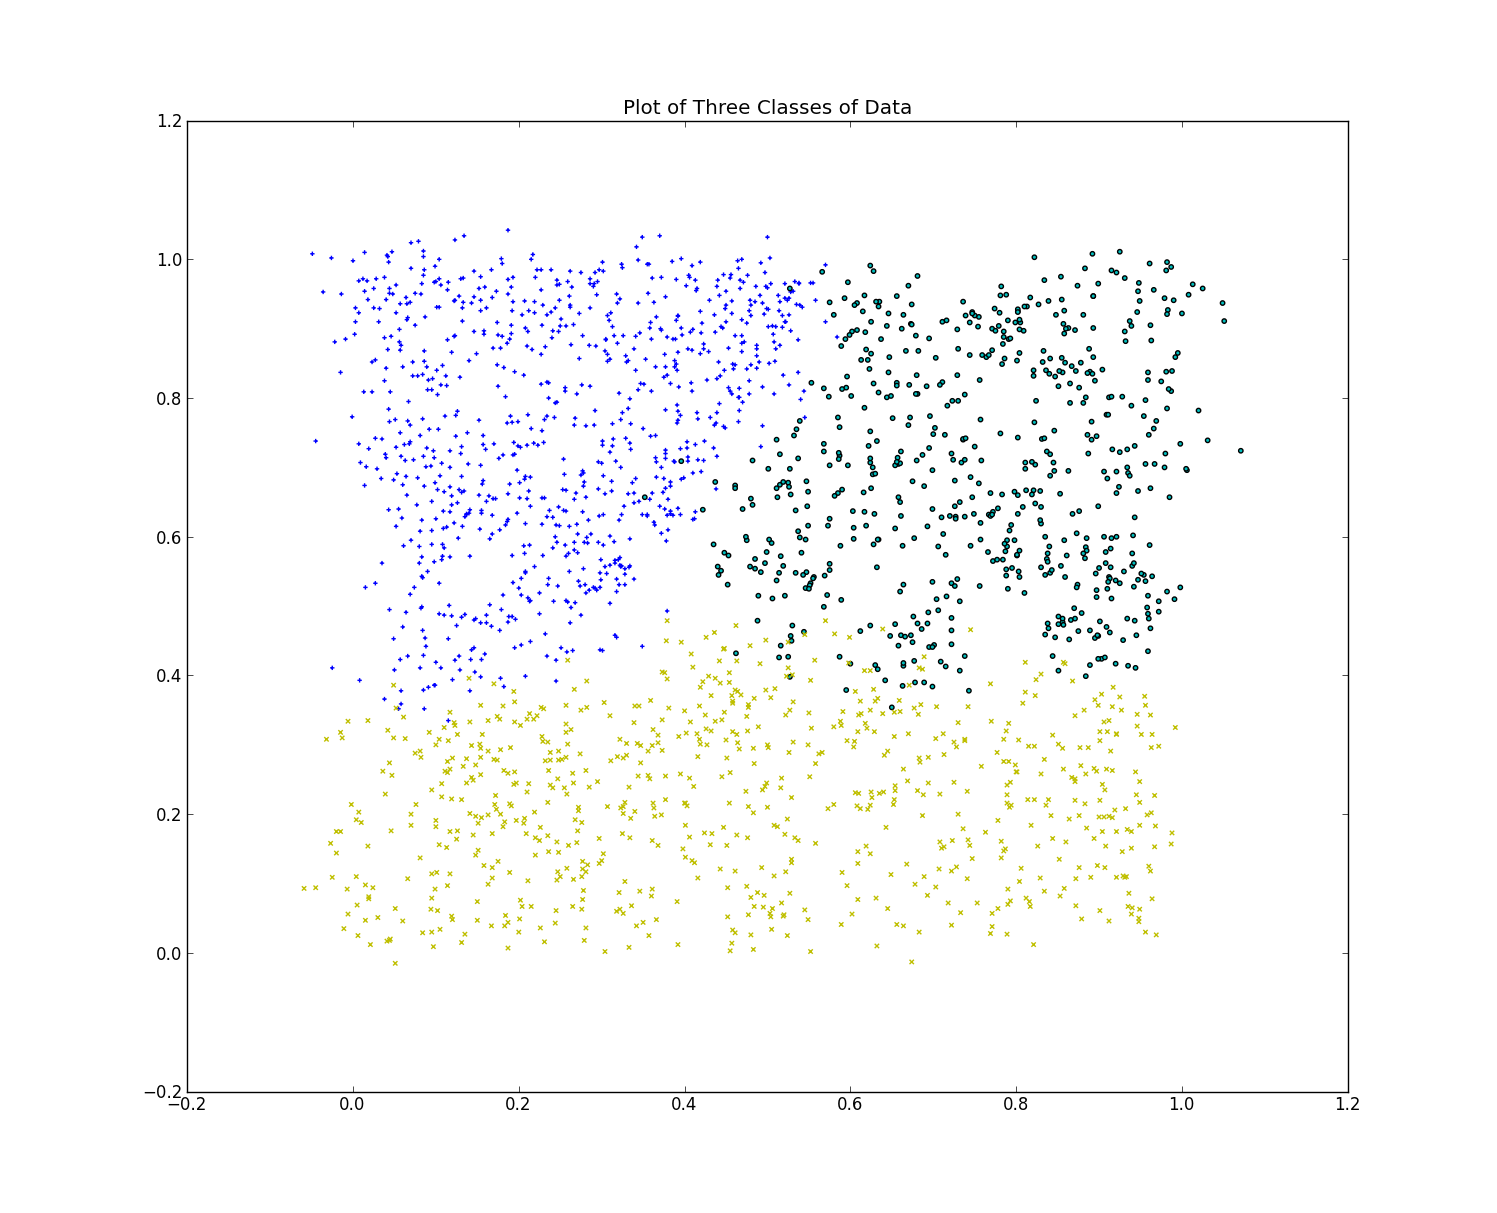
\includegraphics[width=4.5 in]{3_groups.png}
    \caption{Classification of 3 colors in 2-dimensional space}
    \label{Example Data}
\end{figure}

% subsection Overview of Example (end)




% section Assignment One: Overview and Illustrative Example (end)
